\chapter{架构}

\section{ROADMAP}

道法自然

奥卡姆剃刀

PM的质量三角

行百里者半九十

群起而攻之

滚雪球,定义MVP:
\begin{enumbox}
\item \hl{定义存储引擎},用各项特性对设计进行压力测试
\item CRC分析,明确职责,划分模块、定义接口
\item 尽快验证性能、一致性和可靠性
\item 完善自动化测试
\item ***
\item Storage Driver
\item MM
\item ***
\item EC
\item Snapshot
\item Consistency Group
\end{enumbox}

\section{测试}

驱动

网络

perf方式

跟踪每个版本的性能,每个版本都有记录

先验证TCP,测试iscsi、NVMf,导出卷测试。

RDMA

\section{架构设计}

分布式系统架构通常包括几个部分:client、mds、cds。分别对应什么?

vss包括4个range,range包括4个pa,pa包括固定数目的chunk。pa和chunk都是4M大小。
vss是否必要,还是增加了设计复杂度?

token是向range ctl获取的,粒度为chunk。range ctl上每个chunk维护有token计数器。

token里包含了每个副本的位置信息,这是向mds请求得到的。

client并不与mds直接通信。分离fr和mds为两个进程,一是可以指定不同的core;二,便于debug。

diskid是全局的,在etcd上有目录。

\begin{center}
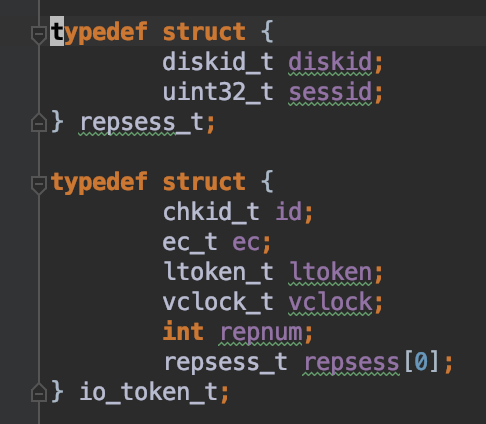
\includegraphics{../imgs/token.png}
\end{center}

问题集:
\begin{enumbox}
\item 为什么range ctl和mds是分离的进程?
\item vss是否必要?
\item ***
\item io路径是什么?
\item IO和Recovery之间如何同步?
\item 副本一致性是如何实现的?
\end{enumbox}

range ctl和mds都在hash ring上。都采用了hash机制来定位目标节点。
ring的节点结构是什么?node and core?
\begin{center}
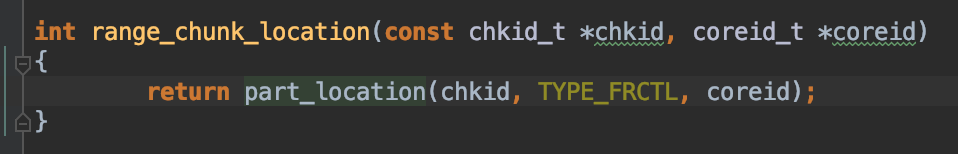
\includegraphics[width=11cm]{../imgs/chunk-location.png}
\end{center}

partition是range ctl和mdctl共用模块。range ctl目前归属frctl。

hash ring上有一个节点充当master角色。如何选主,如何保持其唯一性?
通过etcd lock实现。

lease机制目前没用,如果需要把range ctl放置到session所在的位置,
可以选用lease机制,而不用dht机制。

一旦ring结构发生变化,会有什么影响?SSAN通过epoch来管理ring结构的变化。
ring lock有什么用?

ring上节点负载均匀性如何?

如何识别和处理stale消息?

\section{BACTL}

\subsection{分配}

diskmap.c,不宜放入bactl。bactl所有API都带diskid,针对单盘进行。

数据分布的均匀性、负载均衡

\subsection{Driver}

diskmd磁盘访问接口,支持libnvme驱动。

需要管理物理内存,如hugepage和memory pool。

NVMe/RDMA需要访问物理内存。

\section{Snapshot}

\section{Schedule}

不能支持嵌套task,用pre yield变量来控制。
